\section{Werkzeuge und Technologien}
\subsection{Unterschied zwischen ReactJs und ReactNative}
ReactJs und ReactNative haben zwar sehr viele Gemeinsamkeiten, jedoch auch einige Unterschiede, die vor der Entwicklung mit React Native bewusst sein sollten.
Während ReactJs eine JavaScript-Bibliothek ist, ist ReactNative ein vollständiges Framework. Dies bedeutet, dass bereits beim Setup alles mitgeliefert wird, was für die
Entwicklung notwendig ist. Ein weiterer Unterschied ist der DOM und das Styling. Während die Komponenten in ReactJS meist als HTML gerendert werden, wird bei React-Native
\textit{JSX} verwendet. JSX ermöglicht eine XML-Beschreibung von Komponenten direkt im JavaScript-Code.\\
Der größte Unterschied ist die Plattform, ReactJS ist für Web-Applikationen in Browsern entwickelt. Aus diesem Grund auch der HTML-Code. React-Native ist speziell für Native Applikationen auf
Endgeräten. Aus diesem Grund lässt sich bei React Native auch Nativer Code einbinden. Dies ist leider bei komplexeren Funktionen zwingend notwendig. Um mit den React-Konzepten eine Applikation außerhalb des
Browsers zu entwickeln ist demnach \textit{React-Native} notwendig. \cite{ReactJSvsReactNative:online}

\subsection{Zusammenspiel der Technologien}
In der Vorlesung wurde das Prinzip von React-Native erläutert. In \autoref{fig:ReduxReact} ist 
der grobe Ablauf von React-Native in Ergänzung mit Redux dargestellt. Es ergibt sich ein Kreislauf der beispielsweise durch 
eine Benutzeraktion getriggert wird. Das UI besteht aus Komponenten die jeweils einen eigenen State besitzen. Bei einer Benutzeraktion
triggert UI eine deklarativ beschriebene Action, welche vom Reducer aufgefangen wird. 
Der Reducer kümmert sich unter anderem darum, dass der Store der alle States beinhaltet aktualisiert wird. 
Sobald sich ein State ändert wird das UI neu gerendert und der Benutzer sieht das Ergebnis seiner Aktion. 

\begin{figure}[h]
    \centering
    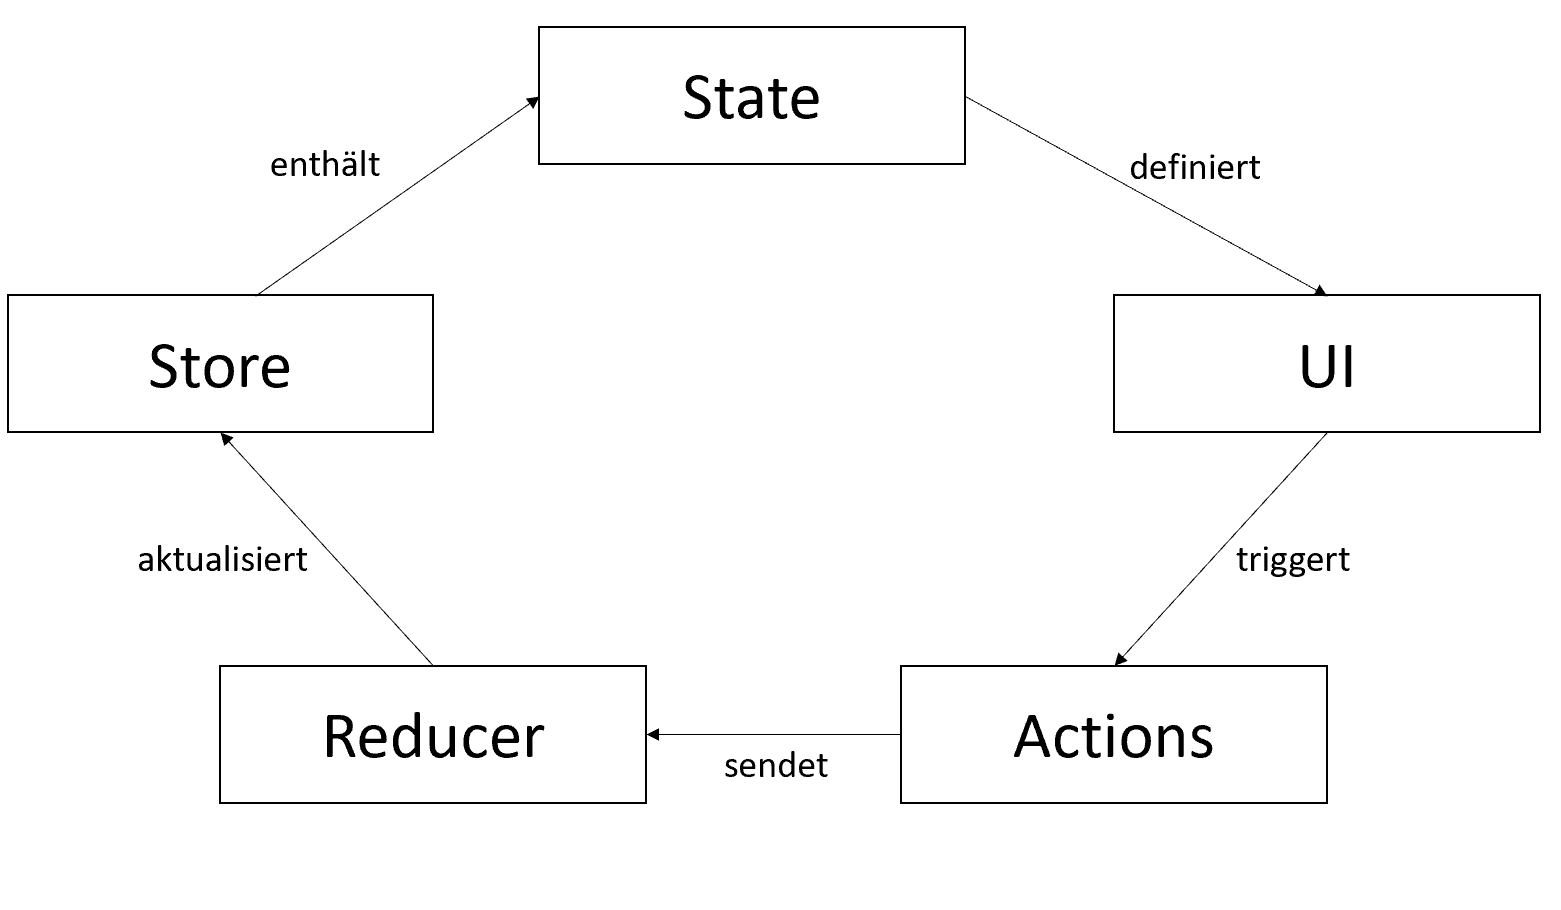
\includegraphics[width=15cm]{ReduxReactGrobAblauf.png}
    \caption{Ablauf: Redux-React}
    \label{fig:ReduxReact}
\end{figure}

Im folgenden werden die einzelnen Komponenten, einschließlich Redux-Saga, erläutert und 
anschließend der detaillierte Ablauf beschrieben. 

\paragraph{Store}
Der Store enthät den kompletten \textit{State-Tree} das bedeutet, dass jede Veränderung 
eines States im Store enthalten ist. Der Store ist damit der zentrale Knotenpunkt der 
Applikation.

\paragraph{Reducer}
Die Reducer sorgen für die Prozessierung der Aktionen. Sie enthalten die Logik, die 
durch eine Aktion ausgeführt werden soll. Sobald eine Aktion getriggert wird, wird diese vom 
Reducer aufgefangen und eine Prozessur die unteranderem den Store aktualisiert wird ausgeführt.

\paragraph{Actions}
Die Aktionen sind rein deklarativ geschrieben. Das bededeutet sie enthalten keine Ausführlogik, 
sondern werden lediglich definiert. Dazu gehört Typ, Interface und Parameter. 

\paragraph{Api}
Die Api enthält Methoden für die verschiedenen Zugriffe auf die Firebase-Datenbank. 
Diese Methoden werden asynchron ausgeführt. Die Api stellt somit die Schnittstelle
zu Firebase dar.

\paragraph{Sagas}
Da die Api-Funktionen asynchron ablaufen, ist für jede Aktion die einen Zugriff auf die 
Datenbank erfordert eine Saga notwendig. Diese strukturiert die Aufrufe und beschreibt, 
die Reihenfolge und triggert \textit{Erfolgsaktionen}. Diese können anschließend im Reducer
verarbeitet werden. 

\paragraph{Components}
Die Komponenten können größtenteils aus den zuvor beschriebenen Bibliotheken verwendet werden. 
Allerdings ist es oft notwendig spezielle Komponenten zu entwickeln. Die Komponenten besitzen 
jeweils einen eigenen State, dieser wird jedoch nur in Ausnahmen verwedet, da das Statemanagement
durch Redux in den Store verlagert ist. Die Komponenten besitzen allerdings \textit{props} über die 
Daten an die Komponente übergeben werden können. 

\paragraph{Container}
Kontainer verküpfen den Redux-State mit dem \textit{props} der Komponenten. Für die Verknüpfung 
kann der Kontainer zwei Methoden enthalten: 
\begin{itemize}
    \item \textit{MapStateToProps}: Diese Methode ist fast immer notwendig, da hier der State mit den \textit{props} verknüpft wird.
    \item \textit{MapDispatchToProps}: Diese Methode ist nur dann notwendig, wenn die Komponente den State verändern kann. Beispielsweise bei einem Input-Field. 
    Die Methode triggert eine Aktion die anschließend vom Reducer verarbeitet werden kann.
\end{itemize}

\paragraph{Screens}
Die Screens gruppieren die Container und stellen diese in einer Oberfläche einem \textit{view} dar. 
Zwischen den Screens läuft die Navigation ab. 

\paragraph{Ablauf von Redux-Saga}
\autoref{fig:ReduxSaga} stellt den Ablauf von Redux-Saga dar. 
\begin{figure}[h]
    \centering
    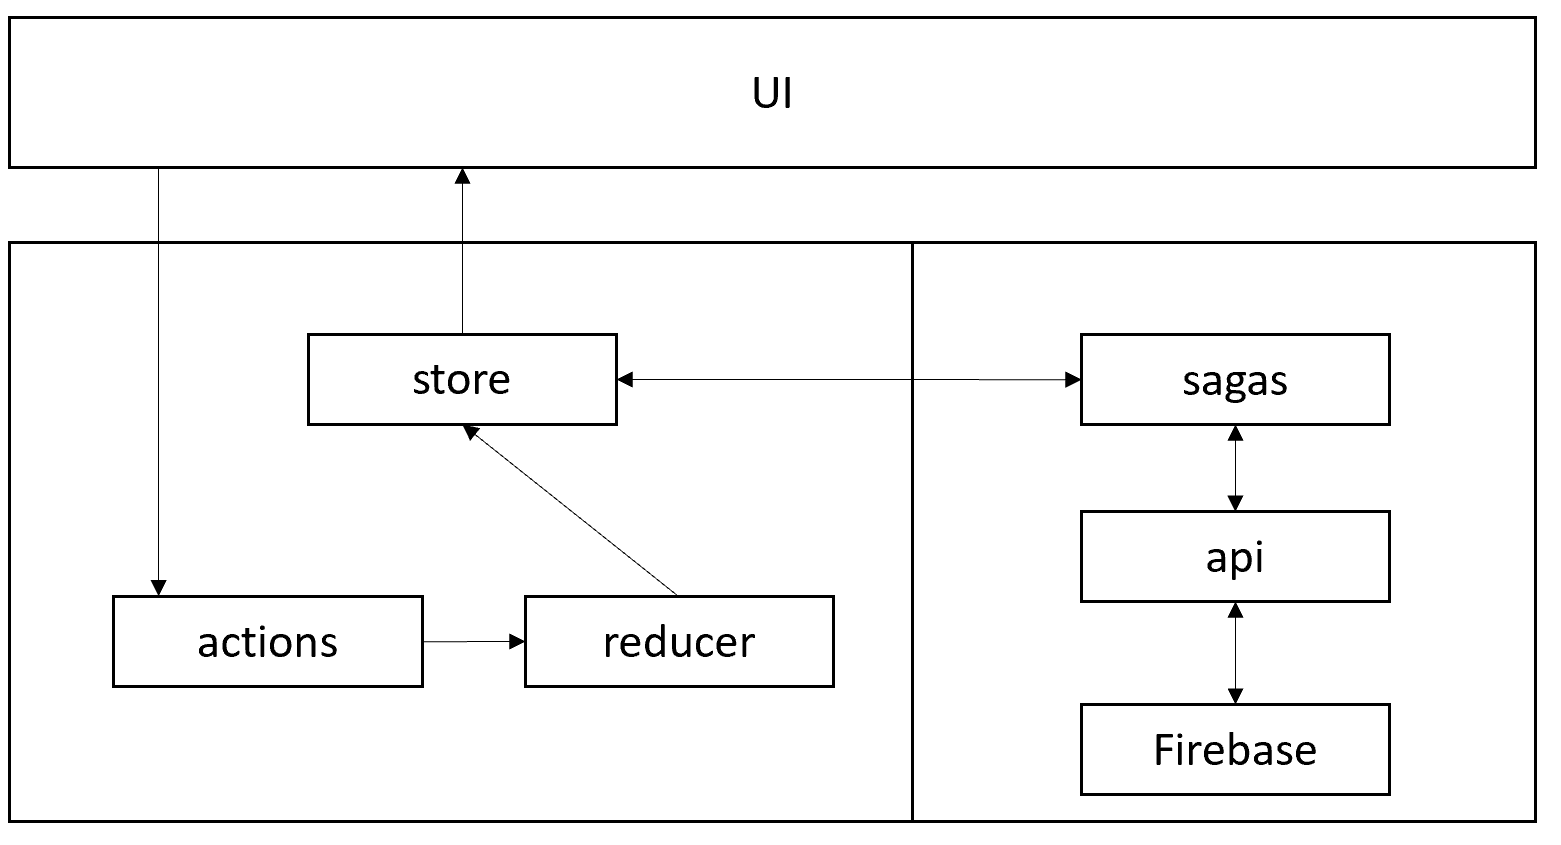
\includegraphics[width=15cm]{ReactReduxSaga.PNG}
    \caption{Ablauf: Redux-Saga}
    \label{fig:ReduxSaga}
\end{figure}

\subsection{Typescript}
Typescript bietet die Möglichkeit typissierten JavaScript-Code zu schreiben.
Durch die Typisierung wird die Entwicklung strukturierter und Objekte werden,
klar definiert. \\
Neben der einfachen Typisierung bietet Typescript weitere Möglichkeiten, die aus
objektorierentierten Programmiersprachen, wie Java, bekannt sind. Dies sind beispielsweise
Interfaces und Klassen. \\
Die Verwendung von Typescript bietet sich bei der Entwicklung von React-Native-Apps an,
da das Framework die Typisierungen sehr gut unterstützt und auch die Unterstützung der React-Native-Community sehr groß ist. \cite{TypescriptReasons:online}

\subsection{Verwendete Bibliotheken}
Im folgenden Abschnitt, werden die in der Applikation verwendetetn Bibliotheken kurz vorgstellt.

\paragraph{react}
Da \textit{React Native} auf React basiert muss die React Bibliothek
in dem Projekt verfügbar sein. Das Konzept und der Ablauf wurde zuvor beschrieben.
Komponenten. \cite{React:online}

\paragraph{react-native}
\textit{React-Native} ist der Renderer, der aus dem JS-Code
die für die plattformspezifische Darstellung benötigten Komponenten erstellt.
\cite{ReactNative:online}

\paragraph{react-native-firebase}
Diese Bibliothek sorgt für eine einfach Anbindung der App zu Firebase. Hier für wird eine leicht-gewichtige
Schicht auf die Firebase SDK erstellt. Durch dieses Paket kann nach Konfiguration sehr leicht mit \textit{firebase.forestore()...}
zugreifen.
\cite{invertas78:online}

\paragraph{react-native-material-dialog}
Native Base liefert leider keinen Dialog im Material Design wird die Komponente zusätzlich als Package
importiert. Dieses Package liefert einen Dialog neben Items für den Inhalt eine \textit{onCancel} und
\textit{onOk},  die die Handhabung des Dialogs sehr simple machen. Der \textit{react-native-material-dialog}
wird in der Applikation für alle vorhandenen Dialoge verwendet.
\cite{MaterialDialog:online}

\paragraph{react-navigation}
Die \textit{react-navigation} bietet eine einfach zu verwendende Navigation für React Native.
Diese Navigation wird in der Applikation für die Navigation über das Menü und für die Navigation
direkt in bestimmte Screens. \cite{ReactNavigation:online}

\paragraph{redux}
\textit{Redux} bietet einen Container für die Verwaltung der States der einzelnen Komponenten.
In einer React-Native App besitzt jede Komponente einenen eigenen State. Um die Verwaltung dieser
States zu vereinfachen, wird Redux verwedendet. Das Konzept von Redux wurde bereits zuvor beschrieben.
\cite{Redux:online}

\paragraph{react-redux}
Dieses Package ist notwendig, um Redux in einer React Native App zu verwenden und so die Vorteile von
Redux zu nutzen. Das Packege verküpft also React Native und Redux.
\cite{ReactRedux:online}

\paragraph{redux-form}
Die Bibliothek \textit{redux-form} unterstützt beim Verwalten der Redux-States in Formularen.
Dem Entwickler werden durch diese Bibliothek sehr viele Schritte abgenommen. Für die Formulare
gibt es einen eigenen \textit{Formreduce}, dieser aktualisiert die zu einer Action gehörenden States.
Der neue Status wird anschließend an das Feld, dass die Aktion gefeuert hat zurück gereicht. Dieser
Ablauf ist in \autoref{fig:ReduxForm} dargestellt. \cite{ReduxForm:online}

\begin{figure}[h]
    \centering
    \includegraphics[width=10cm]{ReduxFormDiagram.png}
    \caption{Ablauf: Redux-Form}
    \label{fig:ReduxForm}
\end{figure}

\paragraph{redux-saga}
\textit{Redux-Saga} wird für asynchrone Aktionen verwendet. Diese finden in dieser
App beim Zugriff auf Firebase statt. \cite{ReduxSaga:online,}

\paragraph{moment}
\textit{Moment.js} ist eine JavaScript-Bibliothek, die das Arbeiten mit Daten vereinfacht. Die Bibliothek ermöglicht es,
ein Datum zu formatieren, validieren und zu manipulieren. Dies ist besonders hilfreich bei der Auswertung und Darstellung der
Zeiterfassung. Das Datum muss hierzu in ein \textit{Moment} umgewandelt werden. \autoref{lst:moment-example} zeigt in einem kleinen Beispiel,
wie die Bibliothek in der Applikation verwendet wurde.\cite{MomentJS:online}
\lstinputlisting[
    caption=Beispiel für Moment.js,
    label=lst:moment-example,
    language=Typescript,
    float=ht
]{moment.ts}'

\paragraph{moment-duration-format}
Dies ist ein Plugin zusätzlich zu \textit{moment.js}. Dieses Plugin in notwendig, da die Dauer ein
grunsätzlich anderes Format hat als ein Datum. Es ermöglicht beispielsweise die Umwandlung einer Anzahl Stunden in Minuten.
In der Applikation wird dieses Format zur Darstellung der Zeiterfassungsergebnisse verwendet. \cite{MomentDuration:online}

\paragraph{native-base}
\textit{NativeBase} ist ein Framework, das eine Schicht über React-Native darstellt. Das Framework bietet,
Komponenten für React-Native, die plattformspezifische Designs umsetzen. Diese Komponenten werden für die meisten UI-Komponenten der App
verwendet. \cite{NativeBase:online}